\section{LOS Coverage Map}\label{sec:los_map}
As a first example the LOS maximum distance will be considered. This, as seen in Section \ref{subsec:los_propagation}, depends on the altitude of the Ground Station and the altitude of the drone. Figure \ref{fig:altitude2distance} shows how the maximum distance in which there is still line-of-sight changes with the altitudes.

However this is not taking into consideration the relief of the Earth's surface, and therefore ignoring the obstacles that one could encounter in the real application. Thus, a more accurate model should be addressed takenb into account the followings:

\begin{itemize}
  \item Terrain elevation
  \item Curvature of the Earth
  \item Altitude of GS and UA
\end{itemize}

\begin{figure}[H]
  \centering
  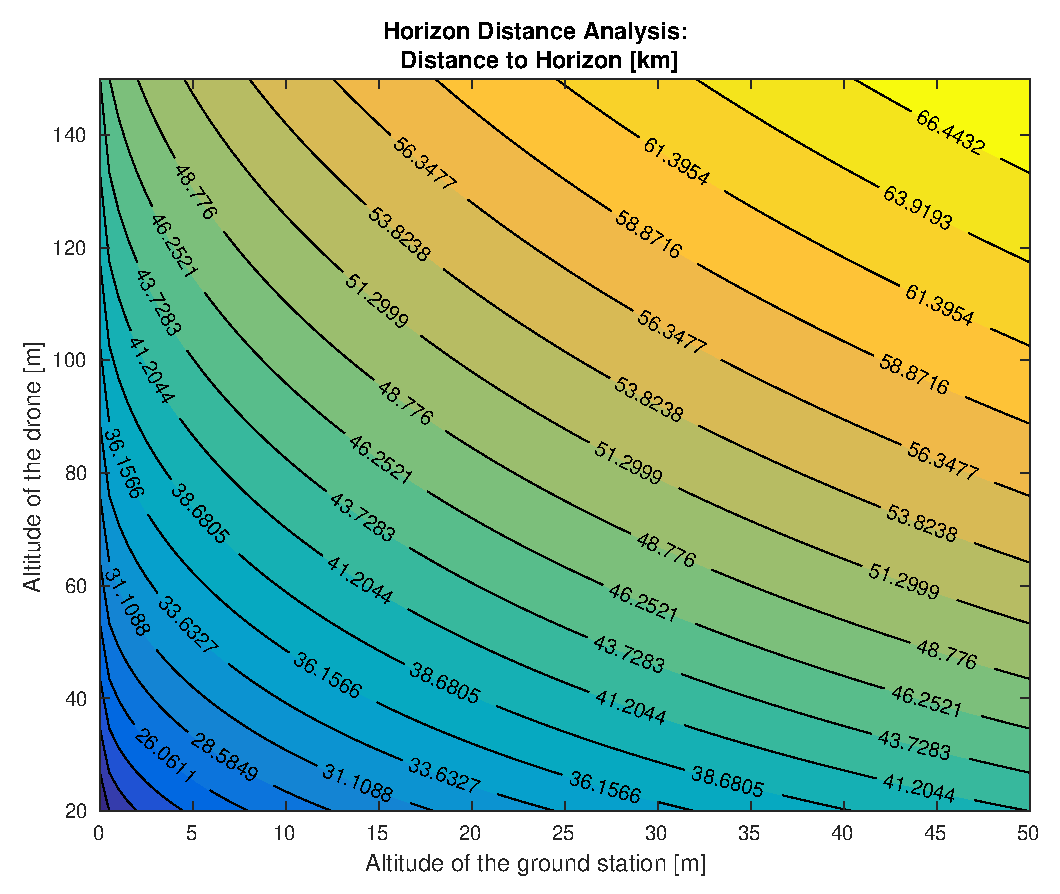
\includegraphics[scale=0.65]{figures/altitude2distance.eps}
  \caption{LOS distance parameter simulation.}
    \label{fig:altitude2distance}
\end{figure}

\subsection{Initial Step}
In this sense, a MATLAB script has been addressed which at first imports a Web Map Service (WMS) in order to load various maps with their topographic data. As example, a map which captures the areas of Denmark and Sweden has been taken along with its terrain elevation as it can be seen in Figure \ref{fig:before_map}.

\begin{figure}[H]
  \hfill
  \subfigure[Map Before Interaction.]{
  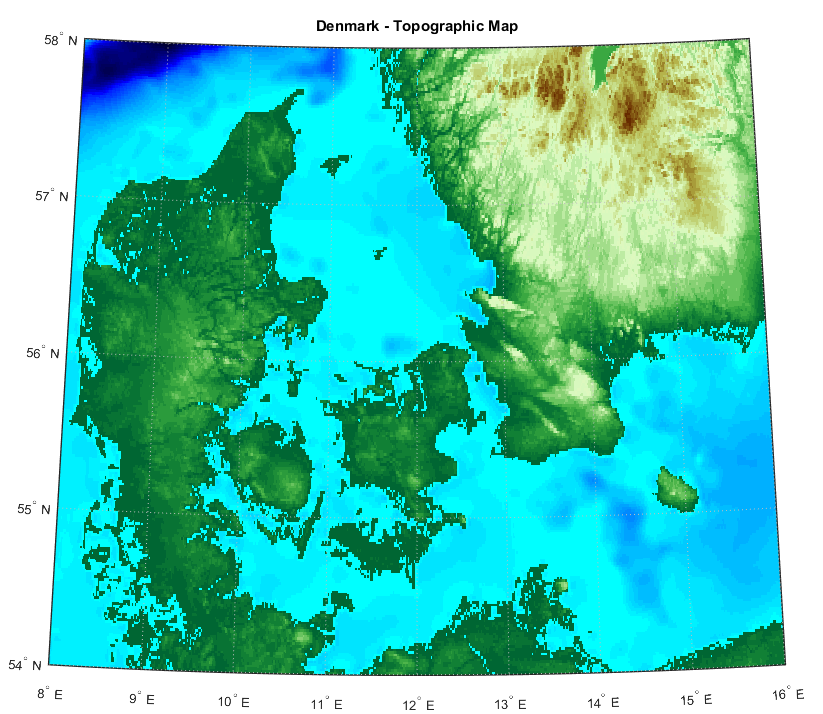
\includegraphics[scale=0.25]{figures/dk_map.png}
  \label{fig:before_map}}
  \hfill
  \subfigure[GS and UA Placement.]{
  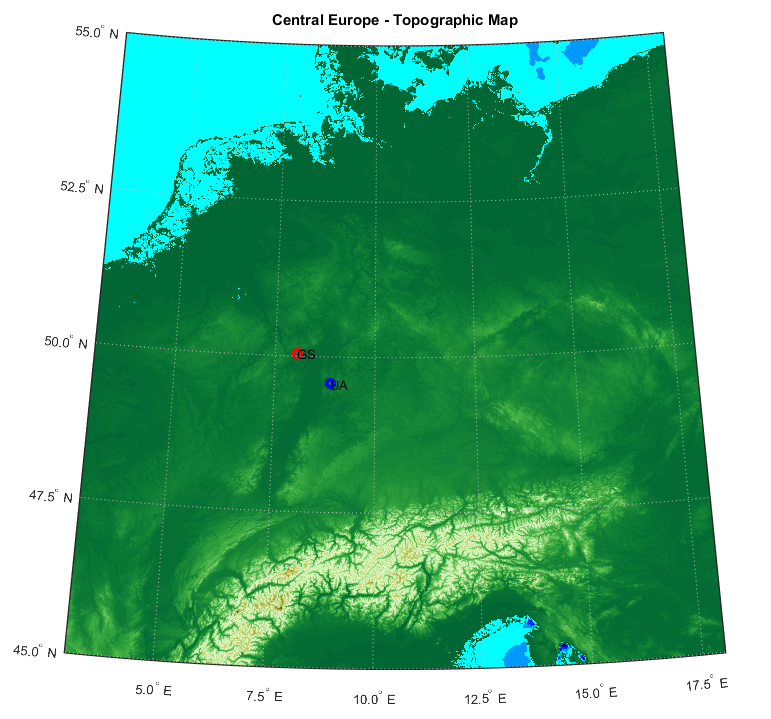
\includegraphics[scale=0.25]{figures/gs_ua_map.png}
  \label{fig:gs_uav_map}}
  \hfill
  \caption{Topographic Map of Northen Europe.}\label{fig:eu_map}
\end{figure}

\subsection{LOS Distance}
Given the map and its topographic data in Figure \ref{fig:before_map}, now it is possible to input the desired points for the GS (orange) and the UA (blue) which gives as result in Figure \ref{fig:gs_uav_map}. The example takes into account the altitude of the GS (20m) and UA (100m) along with the terrain elevation. 

Figure \ref{fig:los_2p} shows the Local NED of the GS (orange cross) perspective which is fixed in zero. Furthermore, the blue crosses and red circles indicate if the UA is visible or not at a particular distance from the GS. Thus, it can be observed that visibility is lost after 50 kilometers from the ground station due to terrain elevation. However, the field of vision is regained between the 55th and 65th kilometer, but the curvature of the Earth comes into play and visibility is lost once again.

\begin{figure}[H]
	\centering
	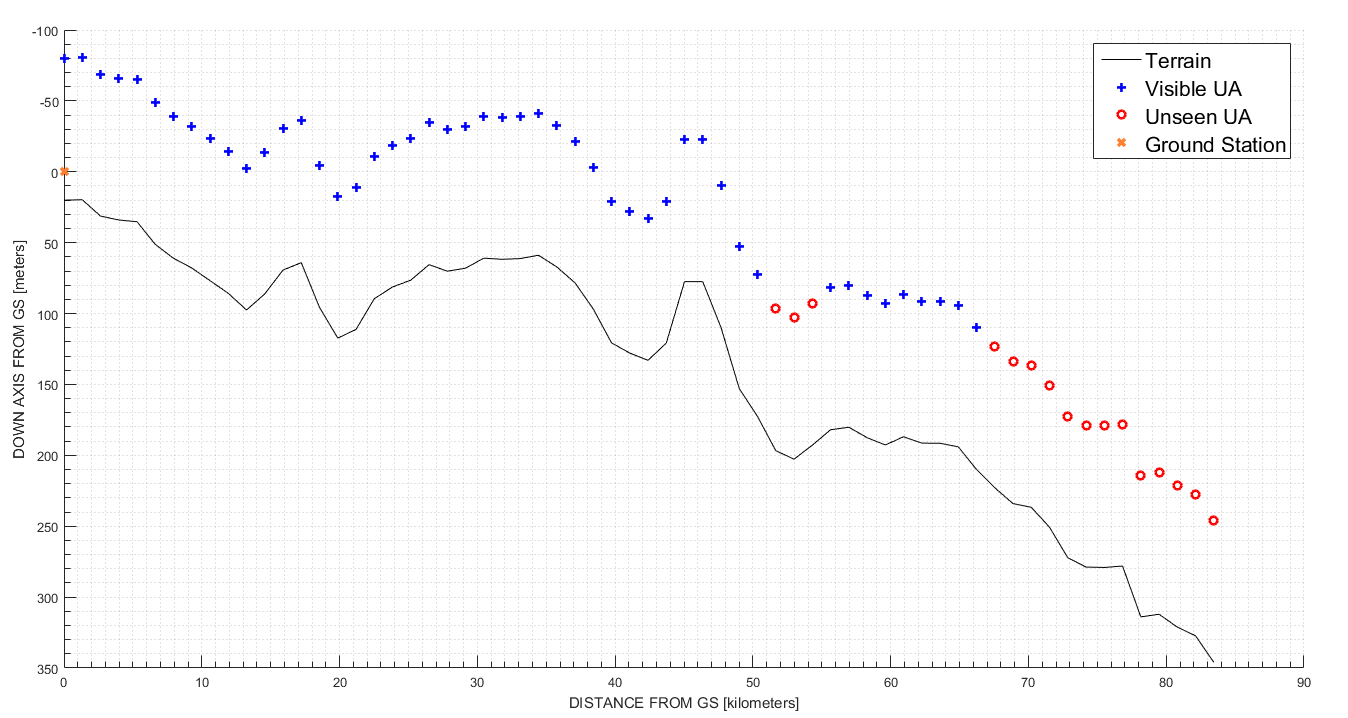
\includegraphics[scale=0.40]{figures/los_2points.png}
	\caption{Line-of-Sight distance seen from the Local NED of the Ground Station.}
   	\label{fig:los_2p}
\end{figure}

\subsection{LOS Coverage Map}
Moving further, for the same map (Figure \ref{fig:before_map}), a location of the GS can be chosen, such that it will result into a visibility area (inside the orange zone) as seen in Figure \ref{fig:los_area}. This area is also referred as the \emph{LOS Coverage Map} and it takes into account the previously mentioned parameters.
It can be observed from Figure \ref{fig:los_area} that in some areas of the map there is no visibility, due to higher terrain elevation or the curvature of the Earth. Additionally, in Figure \ref{fig:los_odense} it can be seen that choosing a good position for the ground station can impact the coverage area, such that the working area of the UAS expands. 

\begin{figure}[H]
  \hfill
  \subfigure[LOS Coverage Map of UAS.]{
  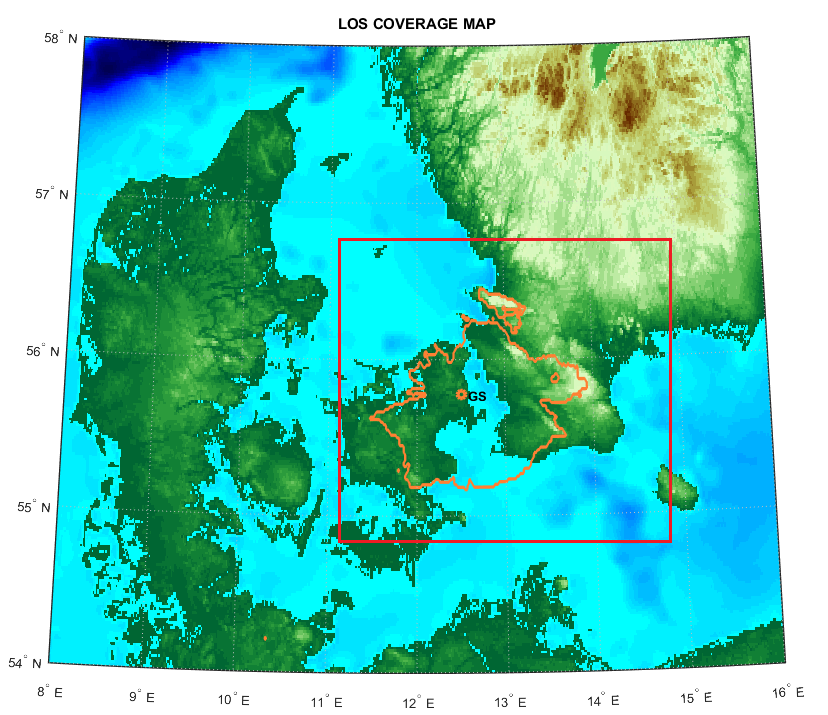
\includegraphics[scale=0.25]{figures/los_area.png}
  \label{fig:los_area}}
  \hfill
  \subfigure[Zoom of LOS Area.]{
  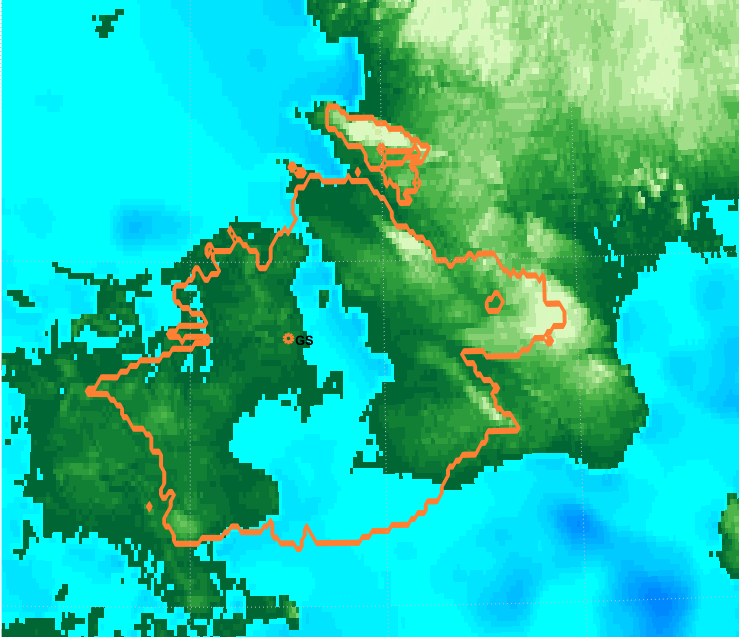
\includegraphics[scale=0.25]{figures/zoom_los_map.png}
  \label{fig:zoom_map}}
  \hfill
  \caption{LOS Coverage Map}\label{fig:eu_map}
\end{figure}

\begin{figure}[H]
	\centering
	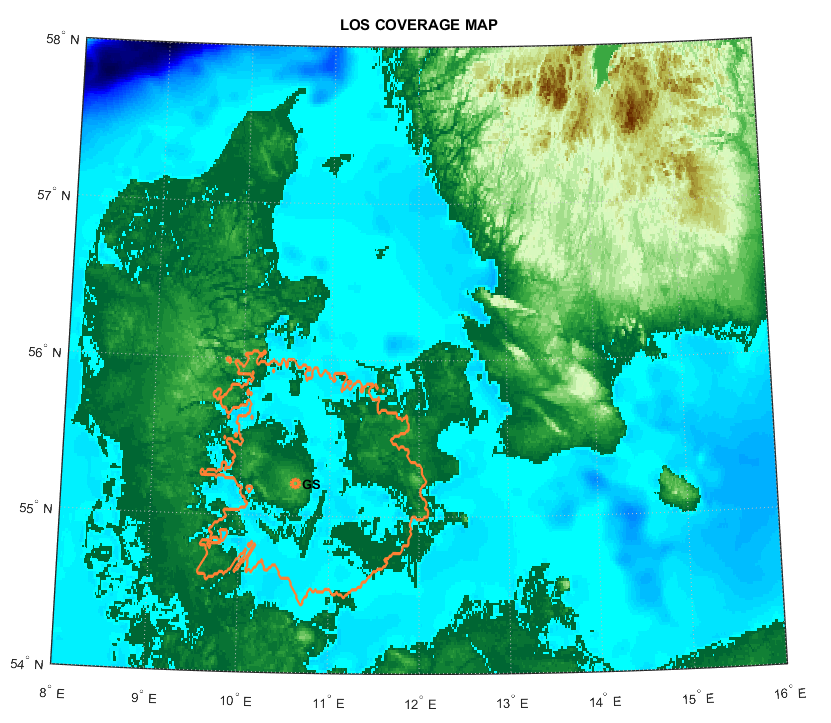
\includegraphics[scale=0.67]{figures/los_odense.png}
	\caption{Example of good GS positioning which impacts coverage area.}
   	\label{fig:los_odense}
\end{figure}

\subsection{Working Principle}
Taking into account that a MATLAB script has been achieved, a thourough working principle has to be addressed in the following steps:
\begin{itemize}
	\item Import topography map 
	\item Input GS and UA altitudes
	\item Choose (click) GS and UA locations on map in order to plot LOS distance
	\item Choose (click) location of the GS in order to plot the LOS coverage map
\end{itemize}